\chapter{Matched Filter}
\begin{center}
	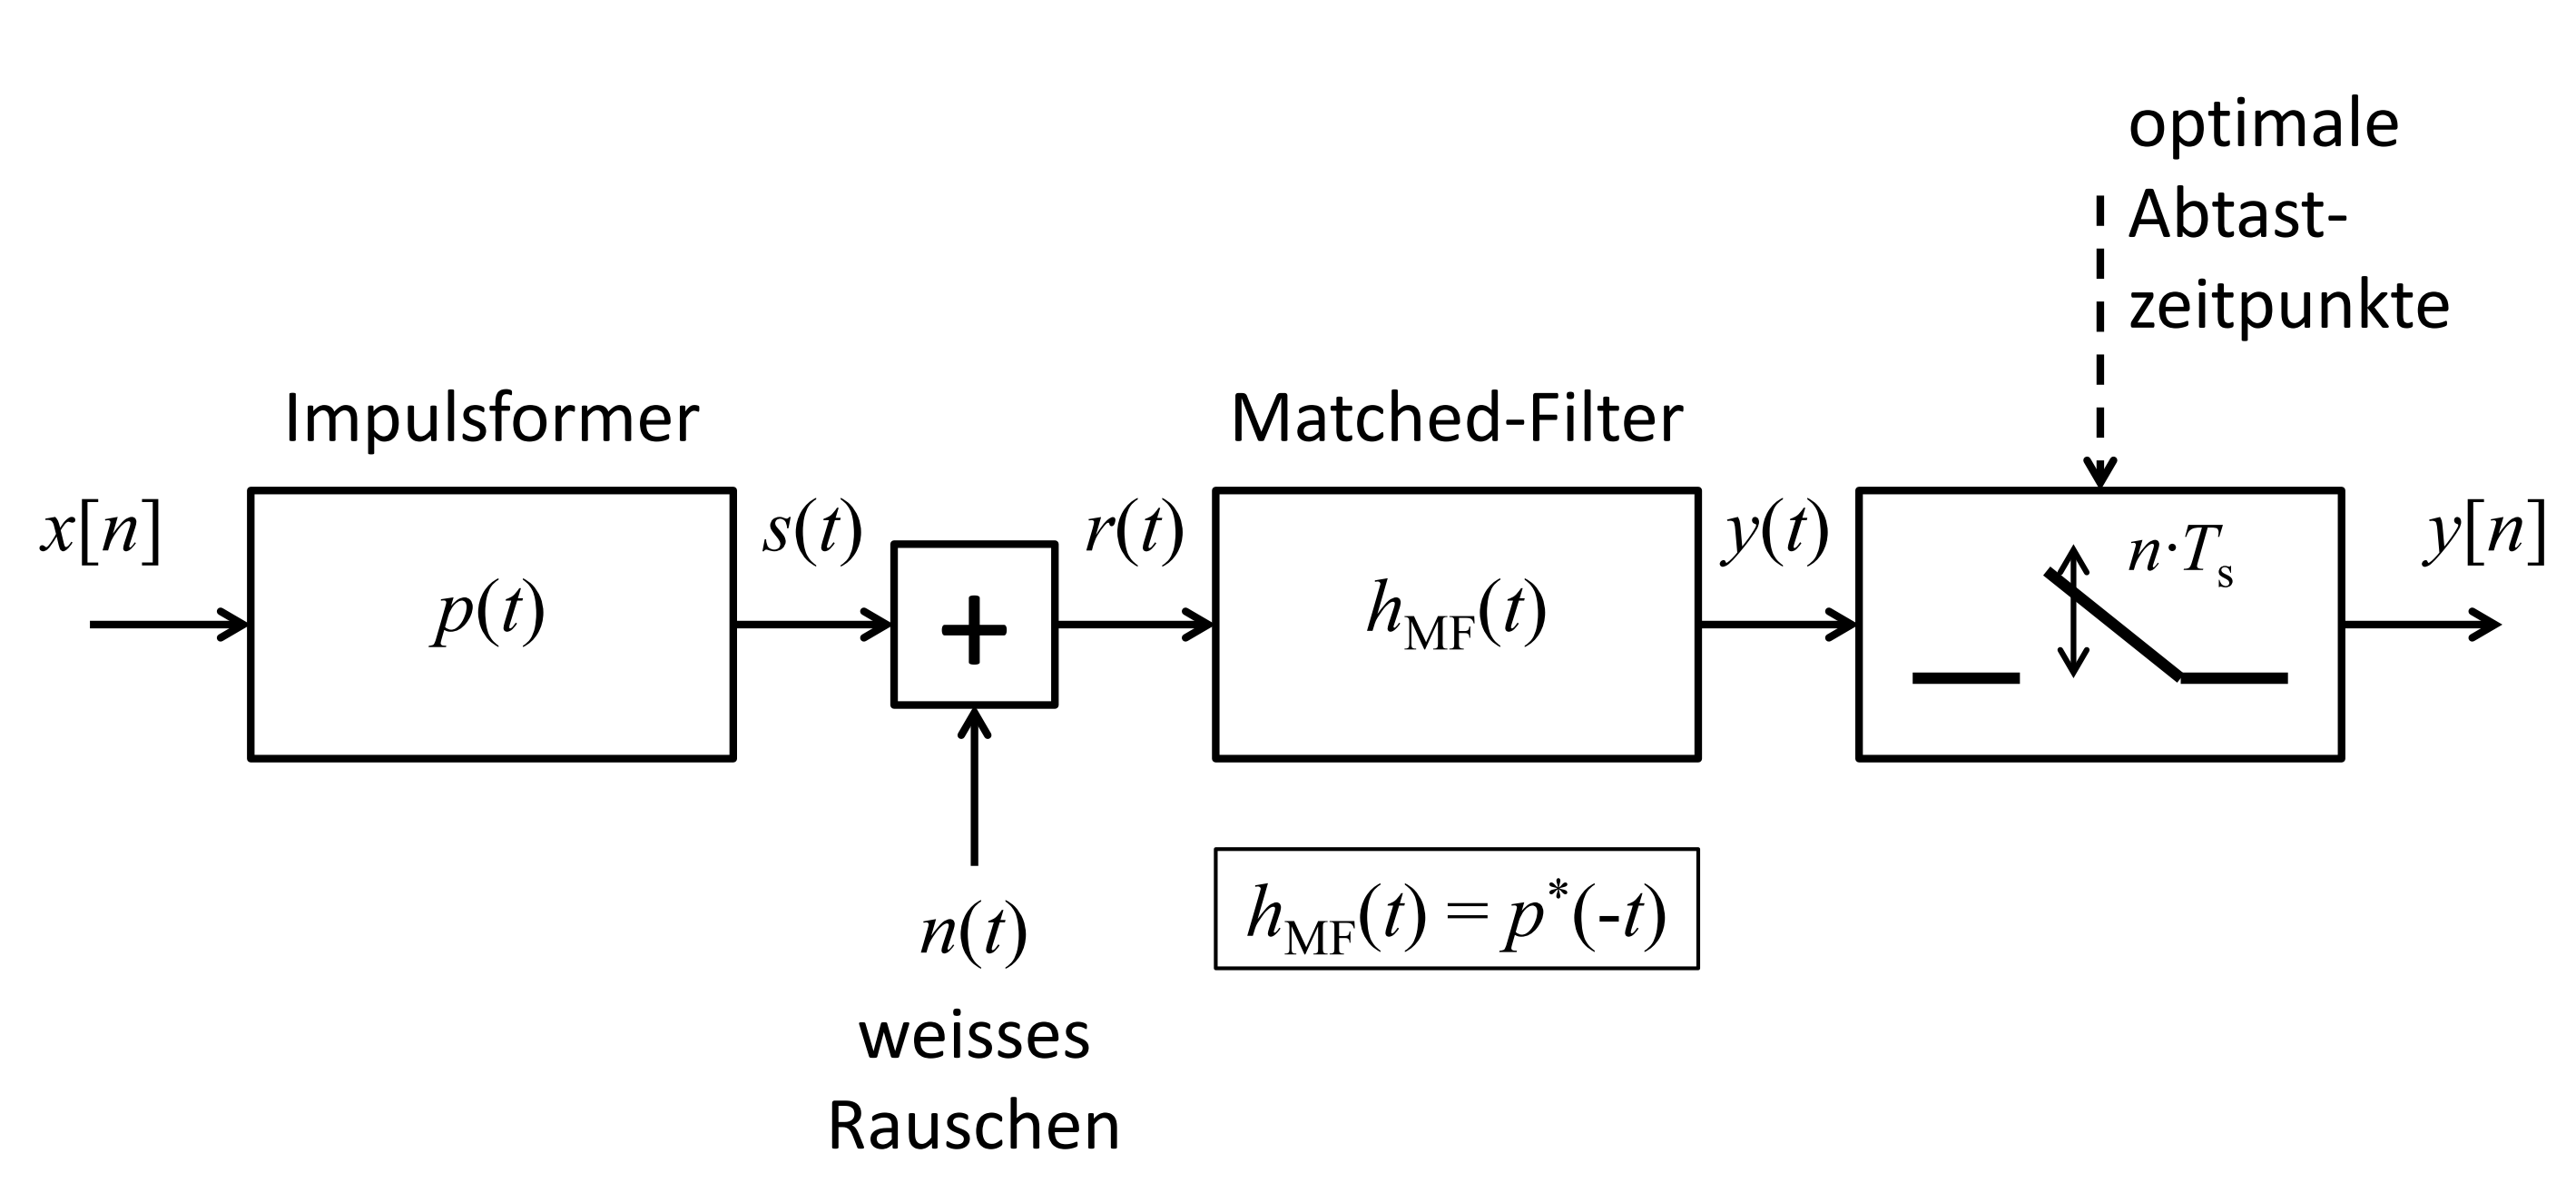
\includegraphics[width=.9\textwidth]{../fig/matched}
\end{center}
~\\
Wahrscheinlichkeitsdichte mit Gauss:
\[
	f_X(x) = \frac{1}{\sqrt{2\pi\sigma^2}}\cdot\e^{-\frac{(x-m)^2}{2\sigma^2}}
\]
~\\
Q-Funktion:
\[
	Q(z) = \int_{z}^{\infty} \frac{1}{\sqrt{2\pi}}\e^{-\frac{x^2}{2}}\di x =
		\frac{1}{2}\textrm{erfc} \left( \frac{z}{\sqrt{2}} \right)
\]
~\\
Error-Funktion:
\[
	\textrm{erfc}(z) = \frac{2}{\sqrt{\pi}} \int_{z}^{\infty}\e^{-x^2}\di x = 2Q(\sqrt{2}z)
\]
~\\
$Y$ ist Gauss-Verteilt mit Mittelwert $m$ und Varianz $\sigma^2$:
\[
	P(Y\geq z) = Q\left(\frac{z-m}{\sigma}\right)
		= \frac{1}{2}\textrm{erfc}\left(\frac{z-m}{\sqrt{2}\sigma}\right)
\]

\section{Weisses gausssches Rauschen am Empfängerfilter}
\begin{center}
	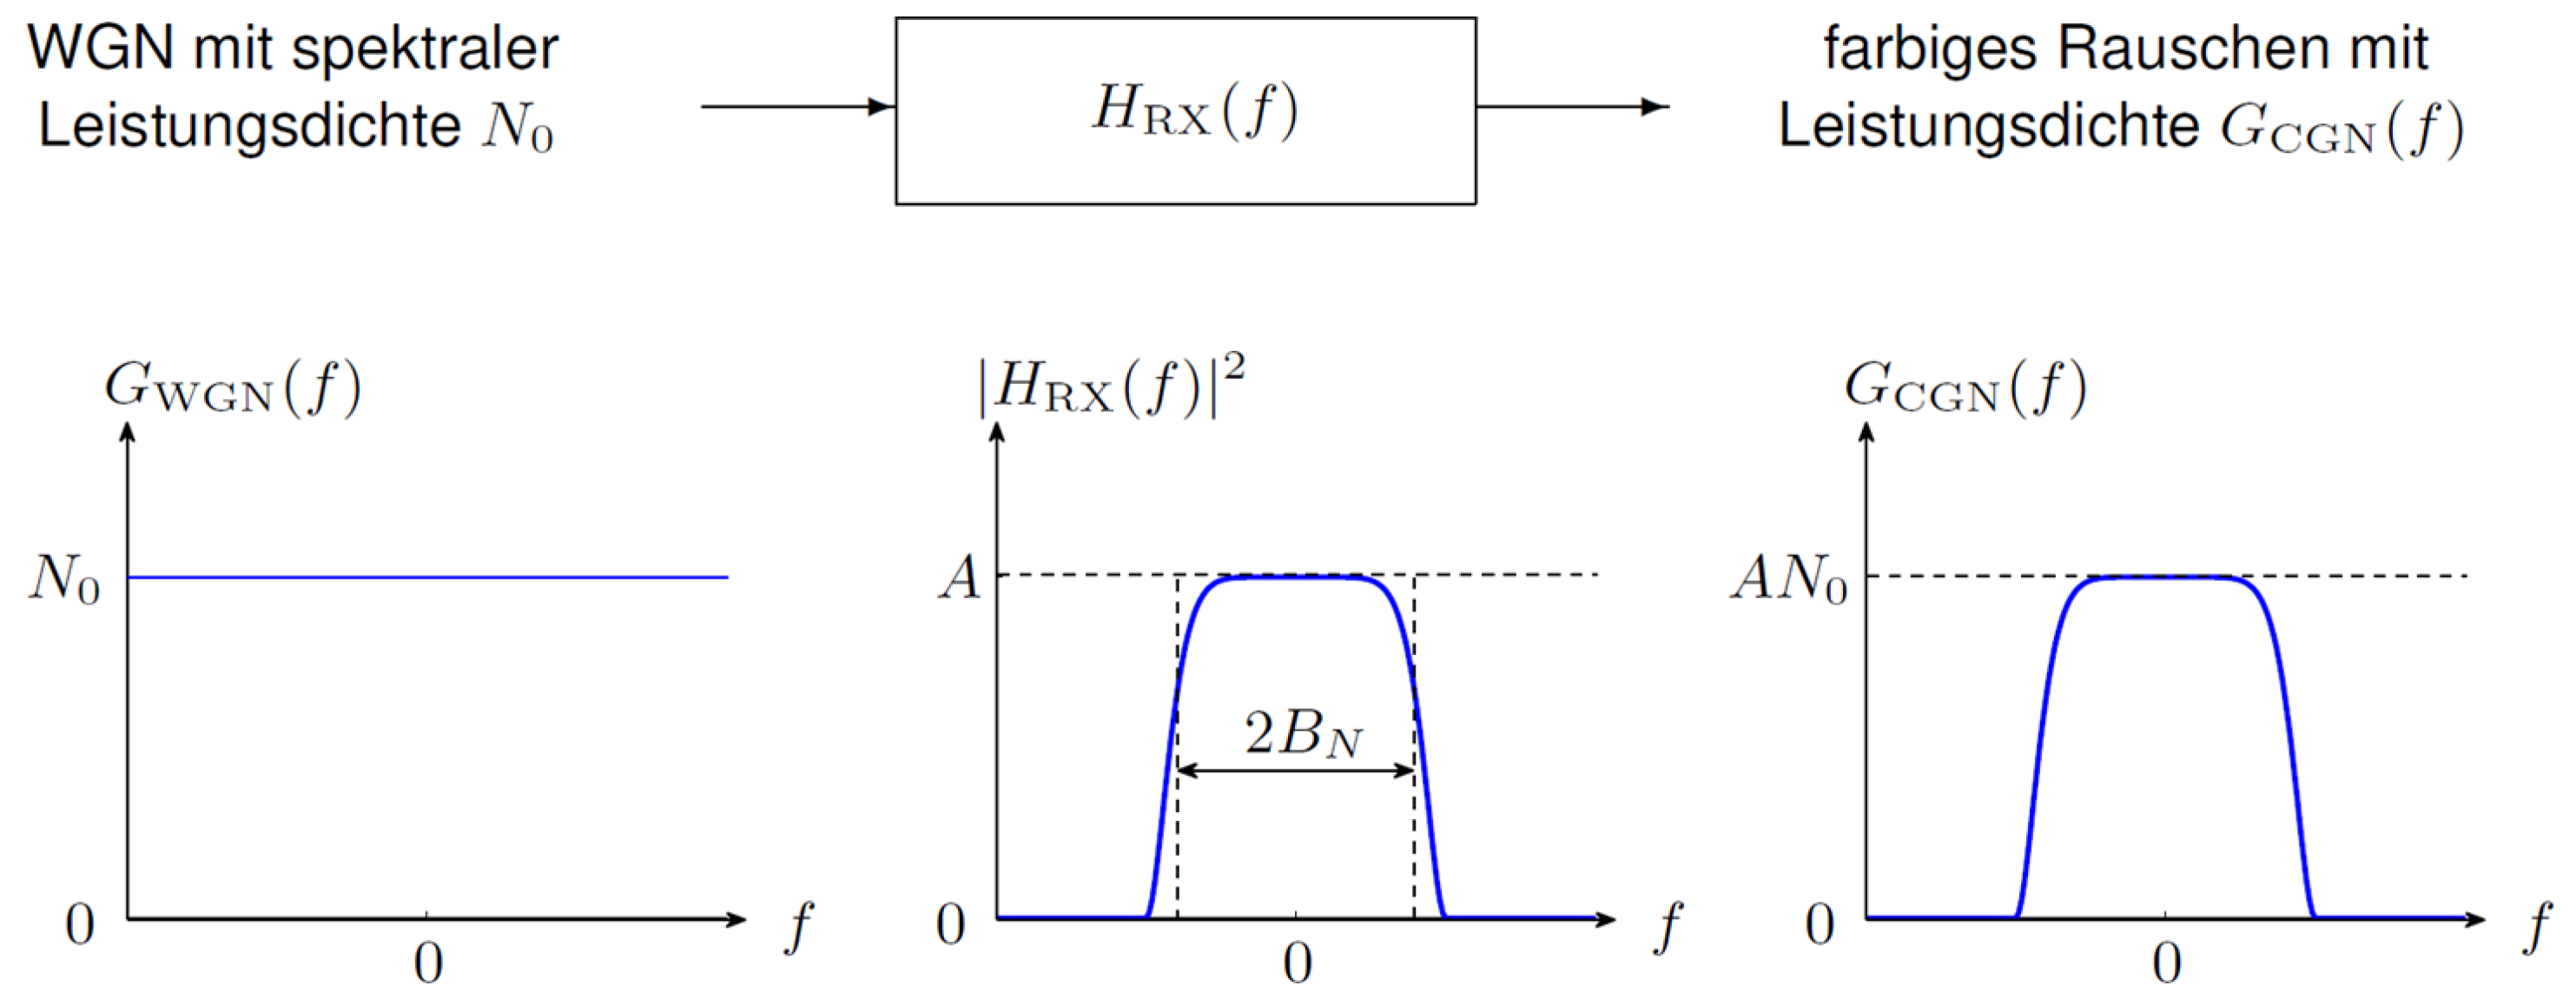
\includegraphics[width=.9\textwidth]{../fig/wgn.png}
\end{center}
Äquivalente Rauschbandbreite des TP:
\[
	B_N = A^{-1} \int_{0}^{\infty}|H_{RX}(f)|^2 \di f
\]
~\\
Leistung des reellen Rauschsignals am Filterausgang:
\[
	\frac{N}{2} = N_0 \int_{0}^{\infty}|H_{RX}(f)|^2 \di f = N_0AB_N
\]

\begin{center}
	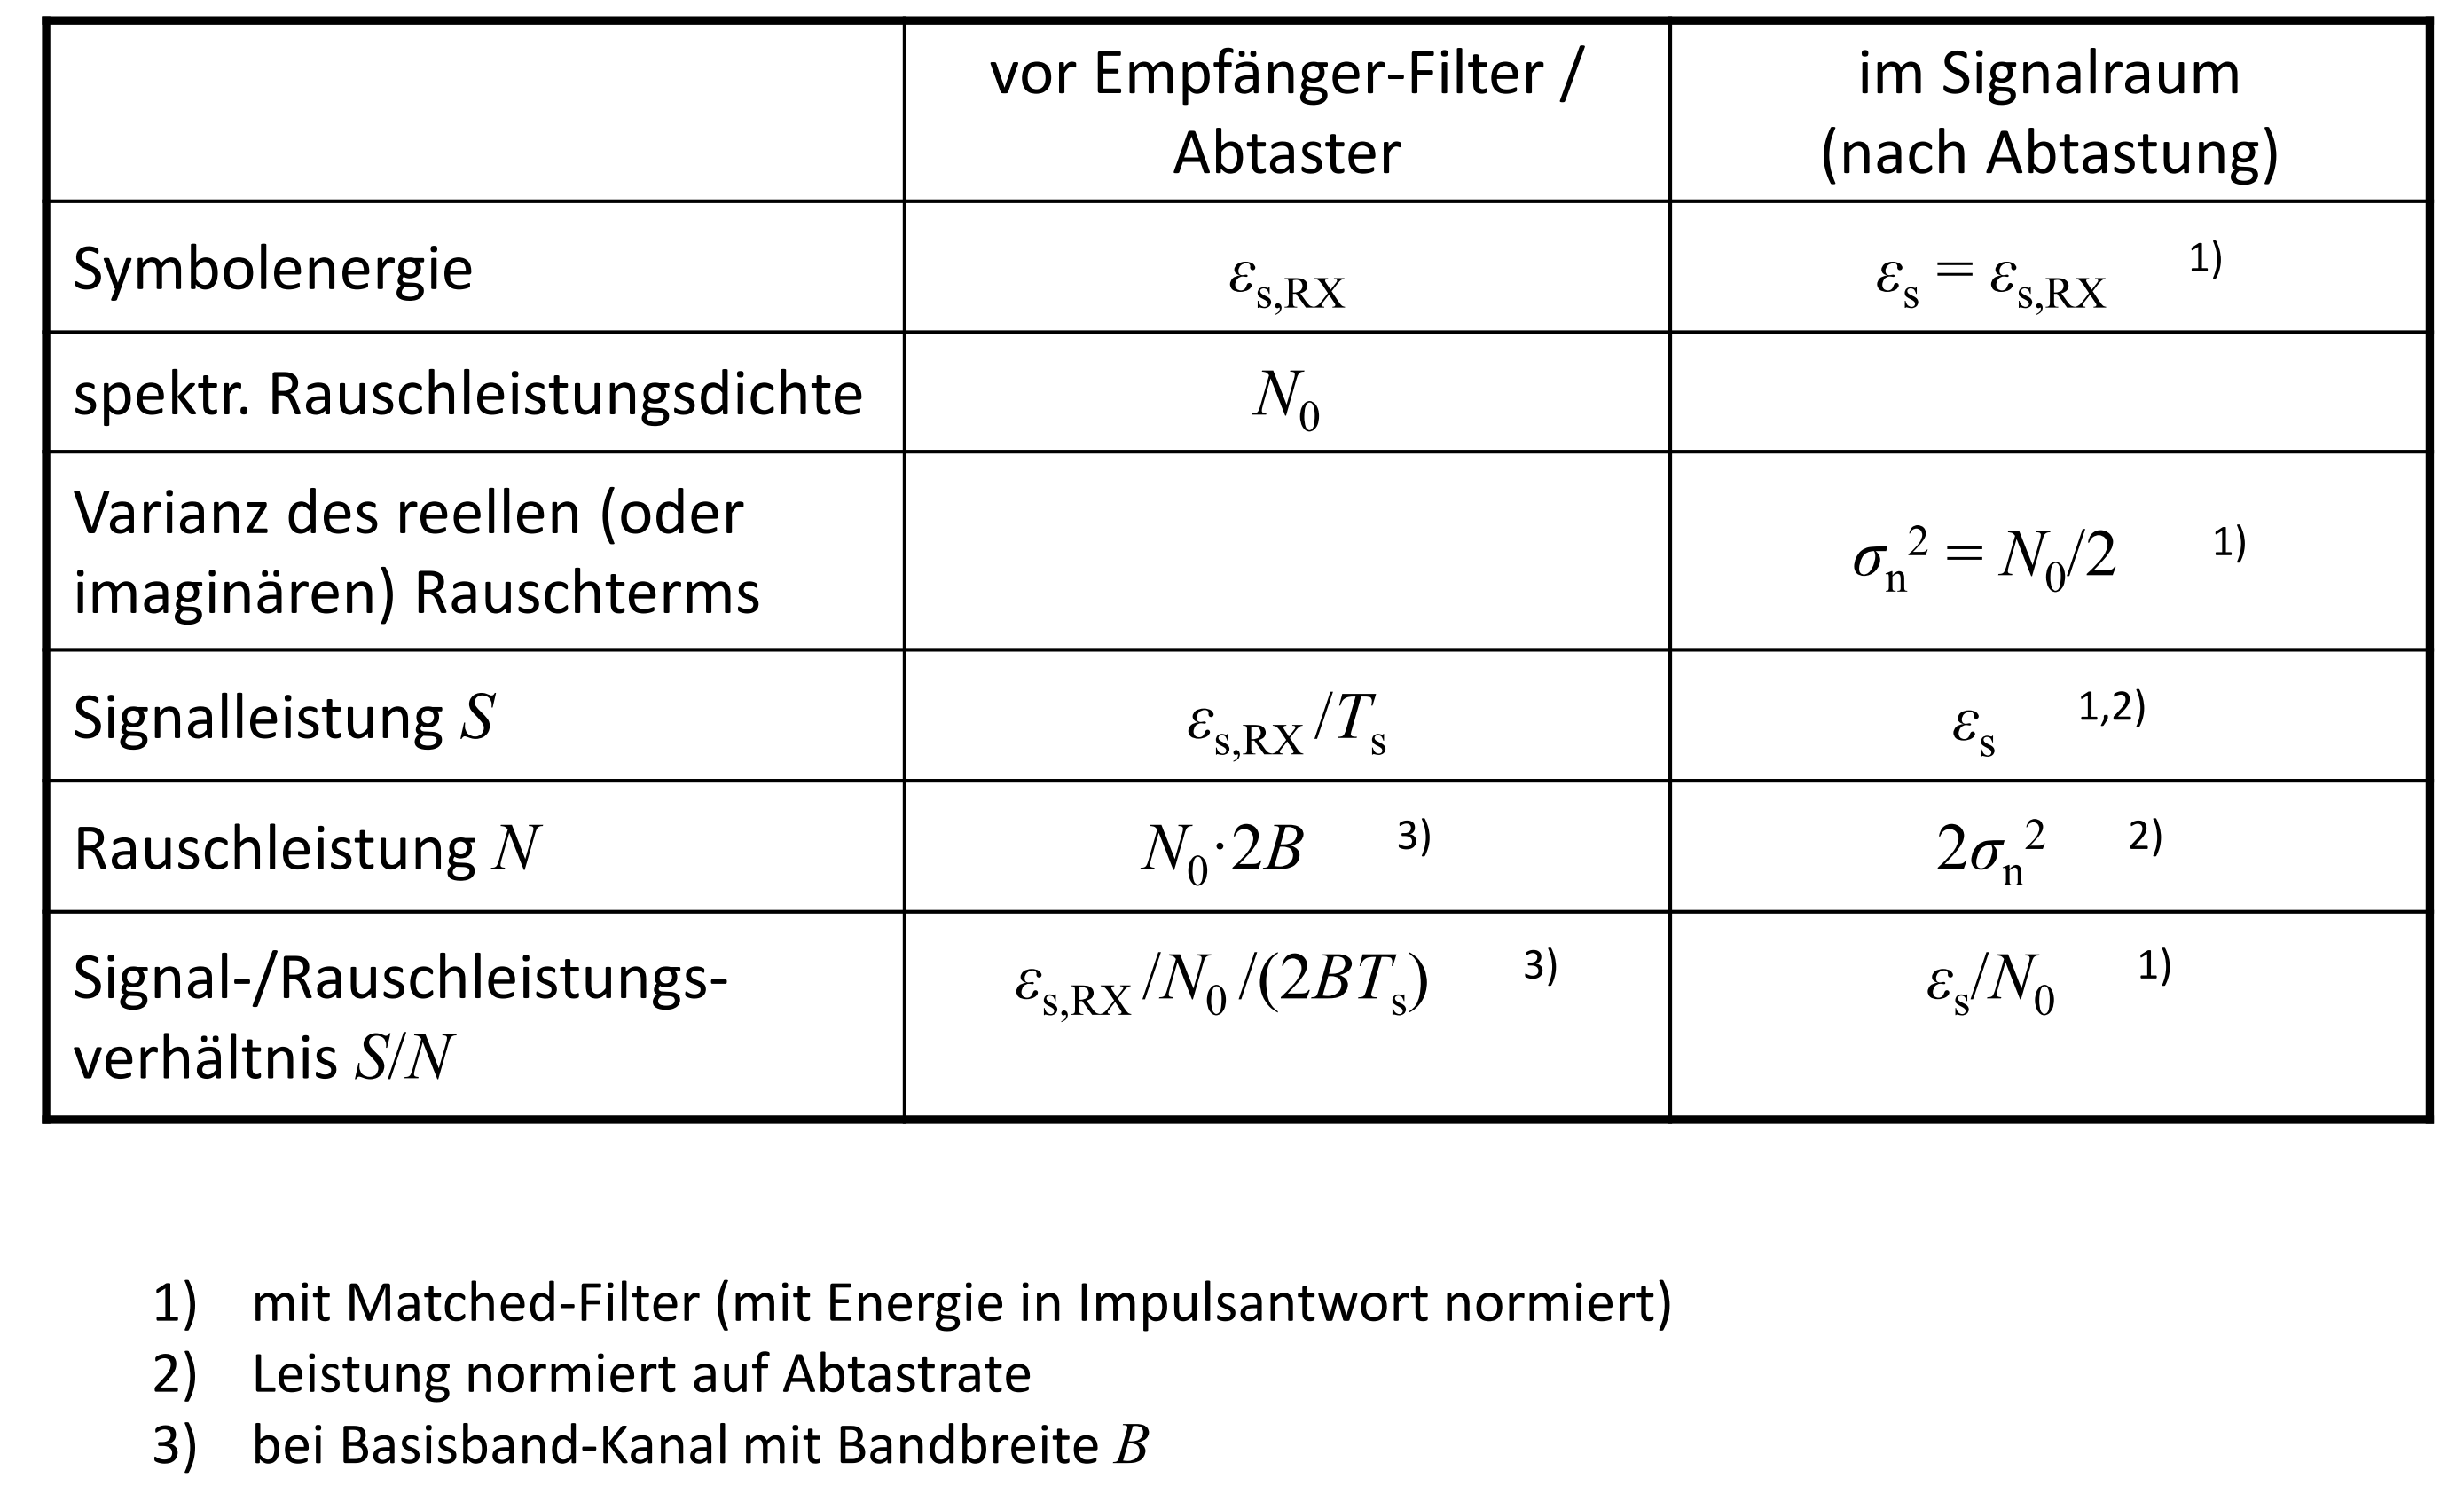
\includegraphics[width=.9\textwidth]{../fig/snr.png}
\end{center}
